\documentclass{thesisreport}
\usepackage{todonotes}
\usepackage{parskip}
\usepackage{graphicx}
\usepackage{float}
\usepackage{multicol} %aggiunto da me
\usepackage{enumitem}
\usepackage{caption}
\usepackage[english]{babel}
\usepackage[utf8]{inputenc}
\usepackage{algorithm}
\usepackage[noend]{algpseudocode}
\usepackage{afterpage}
\usepackage{array}
\usepackage{makecell}
\usepackage{tabularx}

\documentclass[main.tex]{subfiles}
\begin{document}
\begin{center}
\begin{longtable}{ |p{0.8cm}p{6.8cm}|p{0.8cm}p{6.8cm}|  }
 \hline
 \multicolumn{4}{|c|}{Instrumental ADL} \\
 \hline
 \textit{\textbf{Score}} & \textit{\textbf{Activities}} & \textit{\textbf{Score}} & \textit{\textbf{Activities}}\\
 \hline
 \vspace{0.15cm} & & &\\
 
  & \textbf{A. Ability to use telephone}  & & \textbf{E. Laundry}  \\
  
 1 & A.1 Operates telephone on own initiative; looks up and dials numbers, etc. & 1  & E.1 Does personal laundry completely \\
 
 1 & A.2 Dials a few well-known numbers & 0 &  E.2 Launders small items; rinses stockings, etc.\\
 
 1    & A.3 Answers telephone but does not dial & 0 & E.3 All laundry must be done by others.\\
 
 0 & A.4 Does not use telephone at all. & & \\
 
 \vspace{0.15cm} & & &\\

 & \textbf{B. Shopping} & & \textbf{F. Mode of Transportation} \\
 
 1 & B.1 Takes care of all shopping needs independently & 1 & F.1 Travels independently on public transportation or drives own cars. \\
 
 0 & B.2 Shops independently for small purchases & 1 & F.2 Arrange own travel via taxi, but does not otherwise use public transportation.\\
 
 0 & B.3 Needs to be accompanied on any shopping trip. & 1 & F.3 Travels on public transportation when accompanied by another.\\
 
 0 & B.4 Completely unable to shop. & 0 & F.4 Travel limited to taxi or automobile with  assistance of another.\\
 
 & & 0 & F.5 Does not travel at all.\\
 
 \vspace{0.15cm} & & &\\

 & \textbf{C. Food Preparation} & & \textbf{G. Responsibility for own medications}\\
 
 1 & C.1 Plans, prepares and serves adequate meals independently & 1 & G.1 Is responsible for taking medication in correct dosages at correct time.\\
 
 0 & C.2 Prepares adequate meals if supplied with ingredients & 0 & G.2 Takes responsibility if medication is prepared in advance in separate dosage.\\
 
 0 & C.3 Heats, serves and prepares meals or prepares meals but does not maintain adequate diet. & 0 & G.3 Is not capable of dispensing own medication.\\
 
 0 & C.4 Needs to have meals prepared and served. & & \\
 
 \vspace{0.15cm} & & &\\
  
 & \textbf{D. Housekeeping} & & \textbf{H. Ability to Handle Finances}\\ 
 
 1 & D.1 Maintains house alone or with occasional assistance (e.g. “heavy work domestic help”) & 1 & H.1 Manages financial matters independently (budgets, writes checks, pays rent, bills goes to bank), collects and keeps track of income.\\
 
 1 & D.2 Performs light daily tasks such as dish-washing, bed making & 1 & H.2 Manages day-to-day purchases, but needs
help with banking, major purchases, etc.\\

 1 & D.3 Performs light daily tasks but cannot maintain acceptable level of cleanliness. & 0 & H.3 Incapable if handling money.\\
 
 1 & D.4 Needs help with all home maintenance tasks. & & \\
 0 & D.5 Does not participate in any housekeeping tasks. & &\\
  
 \hline
\end{longtable}
\captionof{table}{Instrumental Activities of Daily Living Scale \cite{lawton1970assessment}.}
\label{tab:IADL}

\end{center}
\end{document}
\newcommand\mc[1]{\multicolumn{1}{c}{#1}}
\newcommand\Tstrut{\rule{0pt}{3ex}}       % "top" strut
\newcommand\Bstrut{\rule[-2.6ex]{0pt}{0pt}}   % "bottom" strut
\newcommand\TBstrut{\Tstrut\Bstrut}         % "top and bottom" strut
\setlength{\tabcolsep}{3pt} % Default value: 6pt
\renewcommand{\arraystretch}{2} % Default value: 1
\newcommand{\mySpace}[1][]{\begin{minipage}[t]{\linewidth}#1\end{minipage}}
\setlist[itemize]{leftmargin=*}


\begin{center}
\scriptsize
\begin{longtable}{ @{}m{1.4cm}m{5cm}m{5cm}m{5cm}@{}  }
\hline
\mc{ \small Techniques}\TBstrut & \mc{ \small Pros} & \mc{\small Cons} & \mc{\small Applicability} \\
\hline
\hline
%%Key-Value
 Key-Value &  \begin{minipage}[t]{\linewidth}\begin{itemize}[nosep,after=\strut]
  \item Simple
  \item Flexible
  \item Easy to manage when small size
\end{itemize} \end{minipage} &  \begin{minipage}[t]{\linewidth}\begin{itemize}[nosep,after=\strut]
  \item Strongly coupled with applications 
  \item Not scalable
  \item No structure or schema
  \item Hard to retrieve information
  \item No way to represent relationships 
  \item No validation support
  \item No standard processing tools are avaible
\end{itemize}\end{minipage} & Can be used to model limited amount of data such as user preferences and application configurations. Mostly independent and non-related pieces of information. This is also suitable for limited data transferring and any other less complex temporary modelling requirements. \\ 

%%Markup
 \begin{minipage}[t]{\linewidth} \centering Markup Scheme Tagged Encoding (e.g. xml)\end{minipage}
 &  \begin{minipage}[t]{\linewidth}\begin{itemize}[nosep,after=\strut]
  \item Flexible
  \item More structured
  \item Validation possible through schemas
  \item Processing tools are available
\end{itemize} \end{minipage} &  \begin{minipage}[t]{\linewidth}\begin{itemize}[nosep,after=\strut]
  \item Application depended as there are no standards for structures
  \item Can be complex when many levels of information are involved
  \item Moderately difficult to retrieve information
\end{itemize}\end{minipage} &  Can be used as intermediate data organisation format as well as mode of data transfer over network. Can be used to decouple data structures used by two components in a system. \\ 

%%Graphical
  \begin{minipage}[t]{\linewidth} \centering Graphical (e.g. databases) \end{minipage}&  \begin{minipage}[t]{\linewidth} \begin{itemize}
  \item Allows relationships modelling
  \item Information retrieval is moderately
easier
  \item Different standards and implementations are available.
  \item Validation possible through constraints
\end{itemize} \end{minipage}& \begin{minipage}[t]{\linewidth} \begin{itemize}
  \item Querying can be complex
  \item Configuration may be required
  \item Interoperability among different implementation is difficult
  \item No standards but governed by design principles
\end{itemize} \end{minipage}& 
\begin{minipage}[t]{\linewidth} Can be used for long term and large volume of permanent data archival. Historic context can be store in databases. \end{minipage}\\

%%Object Based
  \begin{minipage}[t]{\linewidth} \centering Object Based\end{minipage}
 & \begin{minipage}[t]{\linewidth}\begin{itemize}[nosep,after=\strut]
  \item Allows relationships modelling
  \item Can be well integrated using programming languages
  \item Processing tools are available
\end{itemize} \end{minipage} &  \begin{minipage}[t]{\linewidth}\begin{itemize}[nosep,after=\strut]
  \item Hard to retrieve information
  \item No standards but govern by design principles
  \item Lack of validation
\end{itemize}\end{minipage} & \begin{minipage}[t]{\linewidth} Can be used to represent context in programming code level. Allows context runtime manipulation. Very short term, temporary, and mostly stored in computer memory. Also support data transfer over network. \end{minipage}\\ 

%%Logic Based
  \begin{minipage}[t]{\linewidth} \centering Logic Based \end{minipage}&  \begin{minipage}[t]{\linewidth} \begin{itemize}
  \item Allows to generate high-level context using low-level context
  \item Simple to model and use easier
  \item Support logical reasoning
  \item Processing tools are available
\end{itemize}\end{minipage} & \begin{minipage}[t]{\linewidth}\begin{itemize}
  \item No standards
  \item Lack of validation
  \item Strongly coupled with applications
\end{itemize} \end{minipage}& 
\begin{minipage}[t]{\linewidth}Can be used to generate high-level context using low-level context (i.e. generate new knowledge), model events and actions (i.e. event detection), and define constrains and restrictions. \end{minipage}\\

%%Ontology Based
  \begin{minipage}[t]{\linewidth} \centering Ontology Based \vspace{0.1 in}\end{minipage}&  \begin{minipage}[t]{\linewidth} \begin{itemize}
  \item Support semantic reasoning
  \item Allows more expressive representation of context
  \item Strong validation
  \item Application independent and allows sharing
  \item Strong support by standardization
  \item Fairly sophisticated tools available
\end{itemize} \vspace{0.1 in} \end{minipage} & \begin{minipage}[t]{\linewidth}\begin{itemize}
  \item Representation can be complex
  \item Information retrieval can be complex and resource intensive
\end{itemize} \vspace{0.1 in}\end{minipage}& 
\begin{minipage}[t]{\linewidth} Can be used to model domain knowledge and structure context based on the relationships defined by the ontology. Rather than storing data on ontologies, data can be stored in appropriate data sources (i.e. databases) while structure is provided by ontologies.\vspace{0.1 in} \end{minipage}\\ \hline

\caption{Comparison of context modelling and representation techniques \cite{perera2014context}.}
\label{fig:ContextModelling}
\end{longtable}
\end{center}

\begin{document}

\thispagestyle{empty}

\def\lskip{\vspace{0.5cm}}


\begin{tabular}{p{7cm}p{10cm}}
ÉCOLE CENTRALE DE NANTES
&
\raggedleft UNIVERSITÀ DEGLI STUDI DI GENOVA	% for EMARO students
\end{tabular}

\vspace{2cm}

% EMARO students
\begin{center} \large\sc MASTER ERASMUS MUNDUS \\ \normalsize{EMARO+ ``European Master in Advanced Robotics''} \end{center}


\begin{center}
	2018 / 2019\\
	\lskip
	Master Thesis Report
	\lskip
	
	Presented by \lskip 
	
	Tommaso Elia \lskip
	
	28/12/2018 \lskip\lskip
	
	{\Large \textbf{Dialogue-based interaction processes with smart homes and companion robots}}
	
	\vfill

Jury \lskip
		
	\end{center}
	


\begin{tabular}{p{3cm}p{6cm}p{6cm} }
 President: & Name & Position (Institution) \\ & & \\ 
 Evaluators: & Name & Position (Institution) \\
	      & Name & Position (Institution) \\ 
	      & Name & Position (Institution) \\ & & \\  & & \\ 
  Supervisor(s):  & Fulvio Mastrogiovanni & Assistant Professor (UNIGE)\\
		  & Enrico Reboscio & Project Menager (DotVocal S.r.l.) \\
		  & Renato Zaccaria & Assistant Professor (UNIGE) \\
(EMARO)  & Co-supervisor from M1 & Position, M1 institution 
\end{tabular}

\lskip

\begin{flushleft}
 Laboratory: Laboratoire des Sciences du Numérique de Nantes LS2N
\end{flushleft}

\newpage
\thispagestyle{empty}
\null
\newpage
\addtocounter{page}{-1}
\pagestyle{fancy}
  
 
\section*{Abstract}
Demographic growth and rise in the average age of the population is increasing the demand for assistance to the elderly.
Ambient intelligence technologies are a response to this demand of supporting the elderly's autonomy.

The work presented in this literature review, is aimed at presenting two problems that are still present in ambient intelligence technologies, i.e., (i) the intrusion in privacy with cameras and (ii) the acceptance of a smart environment by an elderly population.

Furthermore, we show that the integration of a robot companion with cameras and a voice interface, in a smart environment can cope with these problems.

\quad \textbf{Keywords:} \textit{ambient intelligence, companion robot, vocal interface, dialogue management}

 \newpage
 
 %\section*{prova }
 %\newpage
 
 \section*{Abbreviation}
 
 \begin{tabular}{p{2cm}p{12cm}}
 ADL & Activities of Daily Living\\
 AAL & Ambient Assisted Living \\
 IADL & Instrumental Activities of Daily Living \\
 DS & Dempster - Shafer \\
 DL & Description Logic \\
 SWRL & Semantic Web Rule Language\\
 OWL & Ontology Web Language\\
 EMS & Emergency Medical Services \\
 AR & Activity Recognition \\
 IOT & Internet of Things \\
 ML & Machine Learning \\
 TBox & Terminological Box \\
 ABox & Assertional Box \\
 GUI & Graphical User Interface \\
 HRI & Human-Robot Interaction \\
 HCI & Human-Computer Interaction \\
 HMI & Human-Machine Interaction \\
 UTAUT & Unified Theory of Acceptance and the Use of Technology \\
 HAR & Human Activity Recognition \\
 BETA & Black Box Explanation through Transparent Approximation\\
 LIME & Local  Interpretable  Model-Agnostic
 \end{tabular}

 \listoffigures
 
 \listoftables
 
 \tableofcontents
 
 
 \chapter{Introduction}
 %\addcontentsline{toc}{chapter}{Introduction}	 % non-numbered chapters do not appear in table of contents by default

\section{Motivation}
  The demographic growth along with progress of medical technologies results in an increase of elderly population. Indeed in most of the industrialized countries the demographic and social trends have led to greater elderly burden among the population, and that situation critically increases health care demand. Therefore, emergency medical services, public and private health care and patients are subject to more and more stress. 
  In particular, the raising of the average age of the population means higher incidence of chronic diseases that require frequent health assistance and can result in disability and/or lost of independence and deeply affecting health economy for the increasing cost of care. Moreover, if there is a suboptimal management of these diseases there is also an increasing use of Emergency Medical Service (EMS), often avoidable.
 
 In the district of Kaiserslautern, Germany, a significant study was conducted showing that 44\% of Emergency Medical Services (EMS) are dedicated to elderly above 70 years of age \cite{kleinberger2007ambient}.
 	\begin{figure}[H]
		\centering
		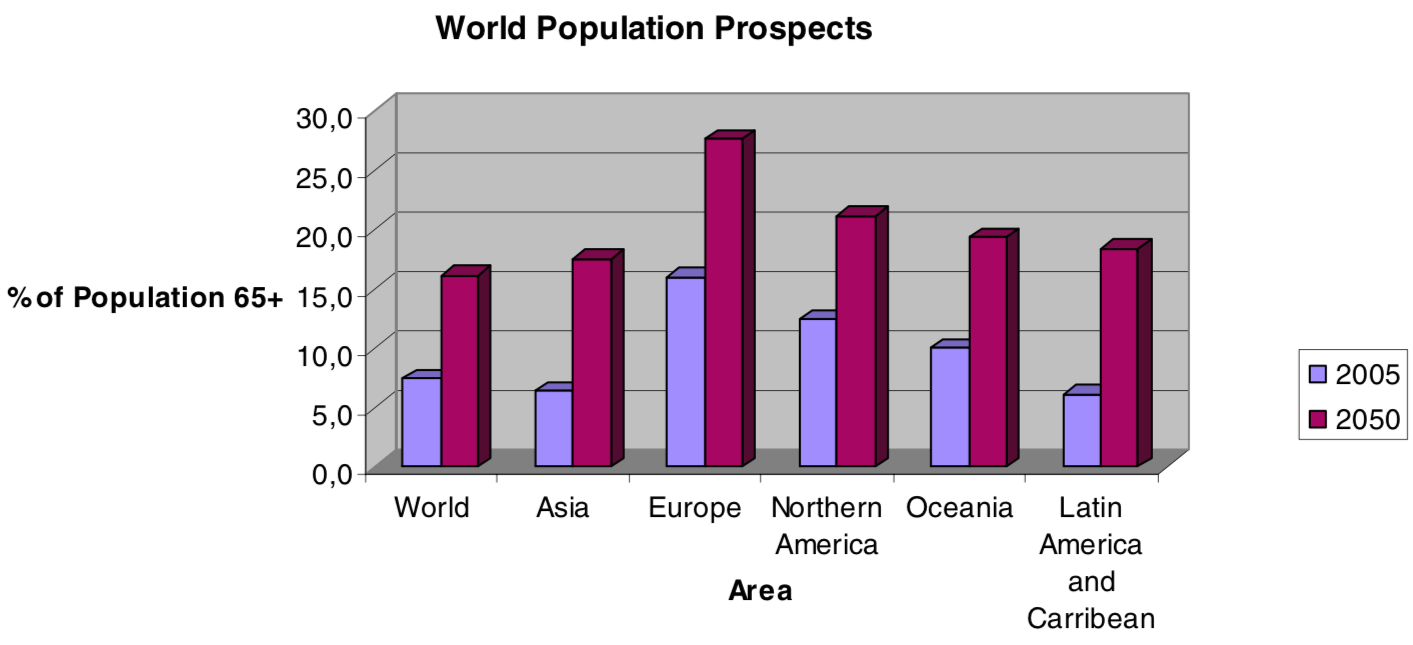
\includegraphics[width=15cm]{Thesis/data/populationProspect.png}
		\caption{\small{Demographical Change according to the United Nations World Population Prospects \cite{kleinberger2007ambient}}}
		\label{fig:populationProspect}
	\end{figure}
 All these elements highlight the increasing cost of health care, the underperforming management of resources and the decline of service quality.
 
 \parskip  \parskip
 
 The Ambient Intelligence technologies help to cope with trends, providing proactive and conscious assistance and supporting the autonomy of the elderly, indeed Assisted Living solutions not only can reduce the costs of managing and monitoring older people but can also offer better \textit{quality of life} \cite{kleinberger2007ambient}.
 
 \section{Context of the Study}
 \label{sec: context of study}
  To guarantee an improved quality of life it is necessary to ensure that the Activities of Daily Living (ADL) are correctly and regularly performed by the assisted \cite{buoncompagni2017towards}.
 
 ADL are defined as daily activities related to motion, rest, nutrition, and personal hygiene, which are a qualitative indicator of person’s wellbeing, determining their quality of life and level of independence \cite{buoncompagni2017towards}. 
 
 At this purpose, in literature the term smart home is used as synonymous of a home that is context-aware. Context awareness has been defined as: ``having information that can be used to characterize the situation of an entity, where an entity can be a person, place, physical or computational object that is considered relevant to the interaction between a user and an application, including the user and applications themselves" \cite{abowd1999towards}.  

 Today, the idea of smart home is deeply changed, especially due to giant stride of the technologies that support it, giving the possibility to create increasingly complex and sophisticated architectures of intelligent environments. At this regard, in the domain of assistive robots and IOT (Internet of Things) field has taken a leading role, also for technological advances in the miniaturization and increased battery life of different types of sensors \cite{phdthesis} \cite{nakashima2009handbook}.
 
 For an easier and immediate comprehension of the possibilities possible by this type of technology, let's have a look to some interesting scenarios that facilitate independence of the elderly individuals:
 \begin{itemize}
     \item \textit{Scenario 1}: The geriatrician with the task of monitoring the health status of elderly could monitor the quality of the patient's sleep through wearable devices or pressure sensors positioned at the base of the bed, visualizing the pattern of sleep during the night;
     \item \textit{Scenario 2}: The system could monitor the daily activities such as getting out of bed, washing and having breakfast etc. and if the patient, for example, stop eating the system warns the geriatrician;
     \item \textit{Scenario 3}: The elder after having woken up decides to take a walk, he puts on his coat and as soon as he crosses the threshold the system realizes that it will  probably rain and the elder has not taken the umbrella risking thus to fall ill. Then the system alerts him via a notification on the wearable device or directly via a voice interface;
     \item \textit{Scenario 4}: The elderly person who is alone at home  and is heading to the bathroom to wash. The system detects his presence in the bathroom and also receives an unclear signal from the wearable he wears that could represent a fall by the elderly. To be certain of the elderly safety, the system could verify it  in two ways: it could ask the elderly about his state through a voice interface or it could send a robot 'companion' to check the situation (for example through image analysis - ML);
\end{itemize}
 
 Smart systems are a very useful reality but it is important not to forget the value of human-human interaction because we do not want that the elderly who are already at a risk of isolation, are further isolated from others, more than before.
 
 \section{Objectives}
 Many elderly people in the last period of their lives need help and special attention but some can not afford a carer economically and others do not want strangers at home. Ambient Home Care Systems can be a solution in this regard, trying, on the one hand, to be as supportive as possible for the daily activities that for the elderly are beginning to be problematic, on the other hand trying to be as less invasive as possible in the life of the elderly trying to maintain their autonomy.
 
 There are many difficulties and challenges in the smart environment, many of them linked to the importance of the general acceptance of the system by the elderly. In fact a lot of solutions currently available put a strong focus on the technological solution and neglect usability issues \cite{kleinberger2007ambient}, which is very important to accept and use the technology that surrounds him.
 
For this reason, the system must meet the following user interface requirements:
 \begin{itemize}
     \item Adaptability: the systems need to adapt themselves to the context at runtime;
     In order to guarantee the best possible service, the system adapts itself according to the situation, for example by scaling down the complexity of the interface in case of emergencies to reduce the cognitive load;
     To do this, the system must be able to monitor the environment around it at all times, to reason on what it perceives and then make the necessary adjustments.
     \item  Natural, anticipatory human-computer interaction: the system must provide different levels of interfaces for different types of users; in particular for the medical and assistance staff, for the operators of the manoeuvring but especially for the assisted persons whose interface must be specially designed according to the their limitations; 
     Indeed the anticipatory interfaces that proactively contact persons in certain situations are considered mandatory.
     \item Heterogeneity: the system must be able to integrate different subsystems supplied by different manufacturers, providing a unique and homogeneous user interface;
 \end{itemize}
 At the same time, however, we need to consider the medical, technological, social constraints and their consequent problems, for example the difficulties for an elderly person to adapt and understand a new technology, or the difficulties of a system to be operative from the beginning.
 
 Given the complexity and the issues typical of an ambient intelligence architecture, the aim of this thesis work is, firstly, to examine a pre-existing architecture by studying its dynamics and by pointing out the underlying strengths and weaknesses. Secondly, this study’s aim is to improve the architecture ability to acquire information also in an equivocal and ambiguous context.
 
 The architecture chosen is called Arianna+ and was developed by Teseo Srl in collaboration with the University of Genova. Arianna+ is a smart home system capable of understanding and making sense of the activities carried out by assisted people, predicting their future behaviours and suggesting personalised healthy habits.
 
 Therefore, in short, the goal is to extend Arianna's AI system as follows:
 \begin{itemize}
     \item Allow Arianna+ to intentionally acquire information when a given context or situation is equivocal, with 2 different approaches:
     \begin{itemize}
         \item By integrating a companion robot with the aim of exploiting its sensors to collect relevant data and by establishing a two-way communication with Arianna’s AI system, which is in charge of processing them and sending back to the robot specific commands;
         \item By integrating a Google Speech API based dialogue management system developed by the company Dot Vocal Srl, where each dialogue is modulated by Arianna’s AI system; 
     \end{itemize}
 \end{itemize}

 The goal is therefore to fit these characteristics in a smart home able to acquire sensory data and save them neatly relying on the context. As result of this approach, a high-level artificial intelligence is able to react also to unclear and uncertain situation, such as scenario 4, through an accurate activities’ detection from the environment and flexible and effective management of saved information.
 
 In this way, the outcome will be an improvement of the system not only functionally but also from the point of view of its usability.
 Indeed, with the integration of a voice interface and a companion robot the user will be encouraged to no longer see the house as a taciturn and hidden entity but as a conscious entity to interact with or a person to talk to in case of need and beyond.
 
\section{Overview of the Thesis}\todo{to correct}
The remainder of the thesis is organized as follows. 

\quad \textit{Chapter 2} presents an overview of the main concepts and techniques adopted in the ambient intelligence field, from the choice of sensors to how and when use them, not forgetting ADL and Ontology definitions that are crucial to understand their role in the following chapters

\quad \textit{Chapter 3} presents the state of the art regarding the topics that are useful to reach our goals:
\begin{itemize}
    \item Section \ref{Arianna}: presents software architecture of Arianna+ and describes the operating mechanisms to manage data from sensors and to recognize elderly activities;
    \item Section \ref{speech}: presents the state of the art for based dialogue management system in smart environment, in particular the possible approaches and solutions that can be adopted in our case;
    \item Section \ref{companionRobot}: presents the state of the art for usage of companion robots in smart environment discussing the advantages and possible choices;
\end{itemize}
\quad \textit{Chapter 4} presents the conclusions reached on the basis of the state of the art presented in \textit{chapter 3}

 \chapter{Background}
The objective of this chapter is to discuss briefly the different aspects that concern smart environment systems:
\begin{itemize}
    \item The type of sensors, that such smart environment systems are  equipped with;
    \item Possible context models to represent a given context based on sensory information;
    \item What are the ADL and how to recognize them;
    \item How to guarantee the reliability of the recognition;
\end{itemize}

 \section{Sensorization}
%  At the base of any smart environment there are devices that make the environment ``smart" which are a group of devices able to exchange between them the formations that detect from the environment \cite{bruno2014public}.
 %% Instead of the above sentence, check out this one:
 Proper sensorization (i.e., in terms of, where to place?, how to acquire and manage sensory data?) plays an important role in making the scenarios described in section~\ref{sec: context of study} a reality. Different types of sensors are at the base of any smart environment system.  Based on the application or the kind of activities that a smart environment intends to recognize; literature shows different approaches for sensorization:
%thetbase of any smart environment there are sensors that \cite{bruno2014public}.
%  In literature it is possible to distinguish two different approaches or modalities for collecting information from the environment:

 \begin{itemize}
    \item On one hand, is the use of \emph{environmental sensors} that detect changes in brightness, temperature, motion, humidity, etc., in the environment. Based on such changes reported over time and detection of interaction between a person and various objects in the monitored area \cite{scalmato2012describing}, a smart environment system can deduce the state of the person inside his/her context \cite{aggarwal2011human}.
    
    \item On the other hand, \emph{wearable sensors} located on a person's body are used to detect changes with respect to the person. In fact with consistent improvement in, the Inertial Measurement Units (IMUs), and their precision in measuring acceleration and orientation of limbs; a wearable sensing system (fig: \ref{fig:Wearables}), is able to monitor body gestures and vital signs \cite{bruno2013analysis}.
 
    \begin{figure}
		\centering
		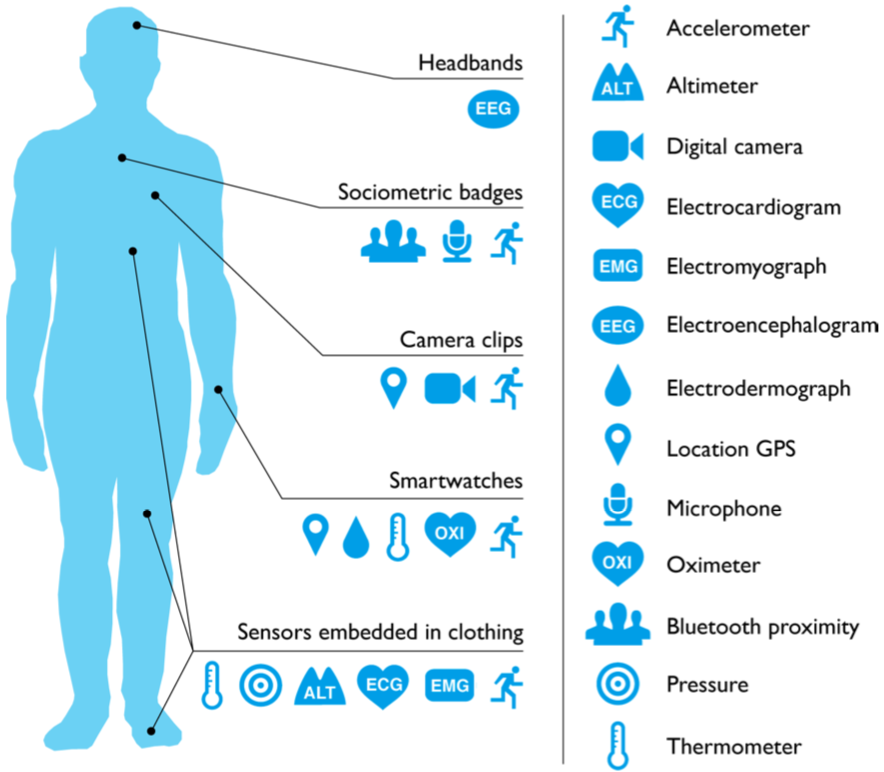
\includegraphics[width=10.5cm]{Thesis/data/sensoring.png}
		\caption{Health Wearables solution \cite{Wearables2016rise}}
		\label{fig:Wearables}
	\end{figure}
	
\end{itemize}

In recent times, there has been massive interest, in combining both the above approaches to detect complex activities based on sequences of simpler activities \cite{bruno2014public, noor2018ontology}. Furthermore for us, based on the scenarios that we wish to accomplish; our smart environment system should be able to detect vital signs, gestures and movements of the person, and also interact with them. Such a smart environment system is said to be context-aware, i.e., it knows the context of the person and interacts accordingly. A context-aware system needs to be modelled, and the process is known as \emph{context-modelling}, which we present further in the next section.

\section{Context Modelling and Reasoning}
\subsection{Context Modelling}
%  There are several popular context modelling techniques, that are used in context-aware computing. However the parameters and factors considered for context modelling are very subjective, as they depend on the application we are building. Chen at al. \cite{chen2000survey} and Strang et al. \cite{strang2004context} discussed the most popular context modelling techniques, each of them having their own strengths and weaknesses that are shown in the table~\ref{fig:populationProspect} below.

The information coming from the sensorization must therefore be organized to represent a context. 
It is necessary to define context information in terms of attributes, characteristics and relationships between different contexts and their evolution over time. The information thus defined compose a context model that must be validated by adding and merging information on the existing context.
There are different techniques of modeling or representation of the context each of them with their own strengths and weaknesses. But the choice of the most suitable model is extremely subjective and related to the application. For this purpose Chen at al. \cite{chen2000survey} and Strang et al. \cite{strang2004context} discussed the most popular context modelling briefly described with the table  \ref{fig:ContextModelling}:
\vspace{0.2 cm}
\subfile{ContextModelling.tex}	

%  As it will be discussed better in section~\ref{ontology}, ontology based approach towards context modelling, is preferred for all its advantages~\cite{perera2014context}

\subsection{Expressivity}

One of the most important features of a representative language or model is expressiveness. It is intuitively used to measure how easy it is for a programming language to implement complex ideas. A model of it is all the more expressive as it is so great the variety and the quantity of ideas that can be used to represent a concept
But it is also important to underline that among the languages presented in the table \ref{fig:ContextModelling}, ontology is without any doubt the most expressive. Unfortunately, more a language is expressive, more the representation of context is complex and computationally expensive \cite{farmer2007chiron}.

 \subsection{Context Reasoning}
 
 Reasoning can be considered as a method to deduce new knowledge based on what is available.  
 The information are processed through reasoning process with the objective to verify the integrity of the data and to establish if the a specific situation occurs. Main approaches towards context based reasoning are discussed in ``Context aware computing for the internet of things:  A survey"~\cite{perera2014context} and are here briefly reported:
 
 \begin{itemize}
     \item Supervised Learning: in this type of technique first we collect a training set examples. Then we label them according to the results we expect. Then we generate the expected results using the training data.
     They are commonly used where the feature set is easily identifiable. Following are examples of models that are based on this technique:\\ \textit{Artificial neural network, Bayesian Networks, Case-based reasoning, Decision tree learning, Support vector machines}.
     
     \item Unsupervised Learning: they are used for situations where possible outcomes are not known. This type of solution has the great advantage of not needing training data. Following are examples of models that are based on this technique:\\ \textit{Clustering, k-Nearest Neighbour}
     
     \item Rule: applicable for situations where raw data elements need to be converted into high level context information. Suitable to use to define events , because it needs for few computational resources and storage. Simple to define and easy to extend.
     
     \item Fuzzy Logic: applicable for situation where it is necessary convert low-level context in to more high-level context information. It is similar to probabilistic reasoning but confidence values represent degrees of membership rather than probability indeed in traditional logic theory, acceptable truth values are 0 or 1. In fuzzy logic partial truth values are acceptable \cite{perera2014context}.
     
     \item Ontology based: It is mainly supported by two common representations of semantic web languages: RDF and OWL. Furthermore, it is based on description logic, which is a family of logic based knowledge representations of formalisms and it is used in case where knowledge is critical and it allows complex reasoning and complex representation basis on the ontology structure. Following are examples of models that are based on this technique:\\ \textit{First-Order Predicate Logic}
     
     \item Probabilistic logic: it allows decisions relying on probabilities attached to the facts related to the problem. It is commonly used where probabilities are known and combining evidence from different sources are essential. Indeed it can handle unseen situations and of uncertainty, combining the evidence. Following are examples of models that are based on this technique:\\ \textit{Dempster-Shafer, hidden Markov Models, naive Bayes}
 \end{itemize}

\subsection{Explainability}
It's necessary to emphasize that each of the different approaches listed before are closely related also with the chosen context model. In fact if for the context model the most important characteristic is the expressivity, for the reasoning process the most important is the explainability, which is the ability to explain or to present model's decisions in understandable terms to a human, as defined by Doshi-Velez and Kim \cite{doshi2017towards}.
Even if we understand the underlying mathematical theories it is complicated and often impossible to get insight into the internal working of the models and to explain how and why a result was achieved.
%To clarify the scope of this survey, we define the explainability of a reasoner as the ability to explain the reasoning of its predictions so that a human can understand. 
Simple rule-based or decision tree approach for instance are more intuitively understandable. The same is not true for approaches as Neural Network or Support Vector Machine which boast high precision at the expense of explainability which can only reached with external models as BETA (Black Box Explanation through Transparent Approximation) \cite{lakkaraju2017interpretable} or LIME (Local Interpretable Model-Agnostic) \cite{ribeiro2016should}.  
It is a very important property because it allows us to fully test and understand the processes that occur in our models.

\section{Ontology} \label{ontology}

According to \textit{Studer et al.} \cite{studer1998knowledge} an ontology is: 
\begin{center}
\textit{``A formal, explicit specification of a shared conceptualisation. A conceptualisation refers to an abstract model of some phenomenon in the world by having identified the relevant concepts of that phenomenon. Explicit means that the type of concepts used, and the constraints on their use are explicitly defined. For example, in medical domains, the concepts are diseases and symptoms, the relations between them are causal and a constraint is that a disease cannot cause itself. Formal refers to the fact that the ontology should be machine readable, which excludes natural language. Shared reflects the notion that an ontology captures consensual knowledge, that is, it is not private to some individual, but accepted by a group.”}
\end{center}

In the ontology based modelling the context is organized into ontologies with different semantic technologies, indeed there are several popular standards (RDF, RDFS, OWL) and reasoning capabilities usable depending on the requirement \cite{perera2014context}. 
In literature it is clear that the current recommendation, for semantic web ontology, is OWL 2 which is an extended version of OWL \cite{perera2014context}. The strength of OWL2 is that it adds more vocabulary for describing properties and classes, which could be used to build complex concepts starting with simpler concepts.
Furthermore, to get the real power of semantic technologies we also use SWRL rules in OWL because they are fully integrated into ontological reasoning. The cons of this approach is that ontologies can becomes exceedingly complex and computationally expensive, slowing down the reasoning process when the amount of data becomes larger and structure becomes too complex.

In conclusion there are several reasons to develop and use ontologies in contrast to other modelling techniques. The most common reasons are that, ontologies allow us to: share a common understanding of the structure of information among people or software agents, analyse domain knowledge, separate domain knowledge from operational knowledge, infer based on high-level knowledge (i.e., making implicit knowledge explicit).

\section{ADL}
Our everyday activities tell us a lot about who we are and how we ensure a certain level of independence \cite{buoncompagni2017towards}. For this reason at first it is very important to define them. As early as late 1950s, we began the study of psychological, social and biological aspects of aging, analyzing the correlation between human actions and cognitive and motor capabilities \cite{buoncompagni2017towards}. 

The Index of Activities of Daily Living, described in \textit{``Multidisciplinary studies of illness in aged persons"} \cite{Multidisciplinary},  is the most used classification of functional status of elderly people and it is based on their ability to execute six different activities that are defined as ADLs (see figure~\ref{fig:indexADL}), i.e., bathing, dressing, toileting, transferring, continence and feeding.

\begin{figure}[H]
	\centering
	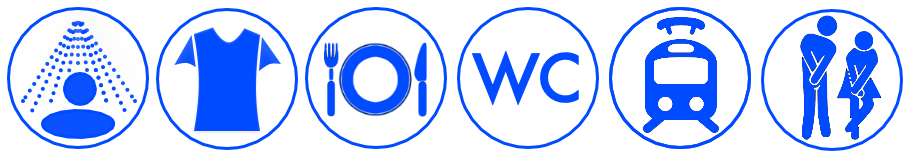
\includegraphics[width=17cm]{Thesis/data/IndexADL.png}
	\caption{Index ADL}
	\label{fig:indexADL}
\end{figure}

 These other eight activities, that take the name of Scale of Instrumental ADL \cite{lawton1970assessment} (IADL), require sufficient capabilities of social skills and planning capabilities using and interacting with everyday objects \cite{buoncompagni2017towards}. 
It takes into account 8 parameters, each parameter in turn can have different degrees of autonomy, for each degree of autonomy it is possible to attract the value 1 or the value 0, for a maximum total of 8 points. This concept can be summarized as shown in the table \ref{tab:IADL}. 

\subfile{IADL.tex}

At the end of the evaluation, by performing the sum of the values you can have a score that varies from 0 to 8.

The value 0 represents total dependence, while the opposite is total autonomy.

It is important to remember that if the non-exercise of an activity is not related to a loss of function but to the fact that that activity has never been performed even when the person was healthy and independent, that specific activity should not be considered to calculate the independence of a person.

Nowadays, as explained in \cite{bruno2014public} the scale of IADL and the index of ADL are the \textit{de facto} standard indexes to evaluate person’s functional status\cite{buoncompagni2017towards}. 

In our case, the term ADL will assume a more general meaning, representing any  considered daily activities, for example, cooking, watching TV etc.
Recognition of ADL falls within the umbrella of human activity recognition (HAR), which aims to recognize the actions and goals of one or more user from a series of observations on the user's actions and the environmental conditions. To this end, there are many systems that attempt to recognize human activities. We explore one such system called Arianna+.


\section{Embodied and Non-Embodied Interface}
 The study of the interaction between human and technology is studied by two complementary research sectors:
 \begin{itemize}
    \item the Human-Robot Interaction (HRI) which can be defined as ``the study of humans, robots and the ways in which they influence each other". As a discipline, HRI concerns the analysis, design, modeling, implementation and evaluation of robots for human use.
    HRI is strongly related to Human-Computer Interaction (HCI) and Human-Machine Interaction (HMI). HRI, however, differs from HCI and HMI because it concerns systems (i.e. robots) that have more complex and dynamic control systems.
     
    \item social intelligence which, in its widest definition, is a person's ability to ``\dots get along with people in general, social technique or ease in society, knowledge of social matters, susceptibility to stimuli from other members of a group, as well as insight into the temporary moods of underlying personality traits of strangers." \cite{vernon1933some}.
 \end{itemize}

 Both play an important role because they both study how much and with which dynamics man relates to the technological system, from the point of view of design and engineering and from the psychological point of view in social intelligence. 
 
 So it is possible to distinguish two opposite approaches. On the one hand, the embodied interface where the social intelligence is managed by a physical piece of technology as a robot (HRI) \cite{lakkaraju2016interpretable, antle2009human, feil2005multi}, in the other hand in non-embodied interface where the social intelligence interface is not longer driven by a robot but by easier communication techniques as vocal interface or a computer (HCI) \cite{antle2009human, feil2005multi}.  


\subsection{Embodied interface}
For embodied interface we mean an intelligent agent that interacts whole with the environment or more specifically with the user through a physical body. Social robots are an example of embodied agents capable of engaging in conversation with one another and with humans employing the same verbal and nonverbal means that humans do (such as gesture, facial expression, and so forth) \cite{serenko2007end}.
\subsubsection{Social Robots}
Social robot means an autonomous or semi-autonomous robot capable of interacting and communicating with human beings or other autonomous physical agents, following social behaviors and rules linked to its specific role. The importance of autonomy in a social robot is clear, since remote controlled robot can be considered a ``simple" extension of the human that controls it. Moreover, an autonomous robot capable of making decisions autonomously has all the requisites to define itself socially \cite{broekens2009assistive}.
 
It's possible to distinguish two different macro types of robots:
\begin{itemize}
\item Human-like: is a robot with its body shape built to resemble the human body like those in the picture \ref{fig:humanoid}. Like us, these robots have a head, a torso, arms, hands and often even legs. But also visual and auditory organs. Humanoid robotics aims to reproduce human beings, our physical abilities, our cognitive processes, our ability to respond to environmental stimuli and adapt to the environment in which we find ourselves. 
\begin{figure}[H]
	\centering
	\begin{subfigure}{0.27\textwidth}
	    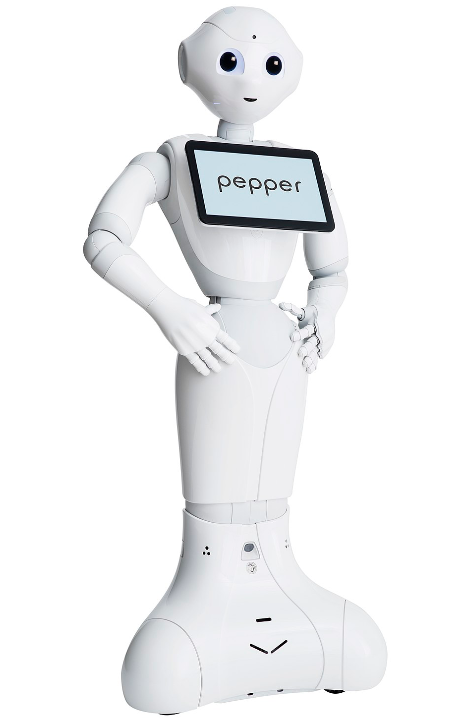
\includegraphics[width=\textwidth]{Thesis/data/pepper.png}
         \caption{\centering Pepper robot of SoftBankRobotics}
        \label{fig:pepper}
	\end{subfigure}
	\begin{subfigure}{0.27\textwidth}
		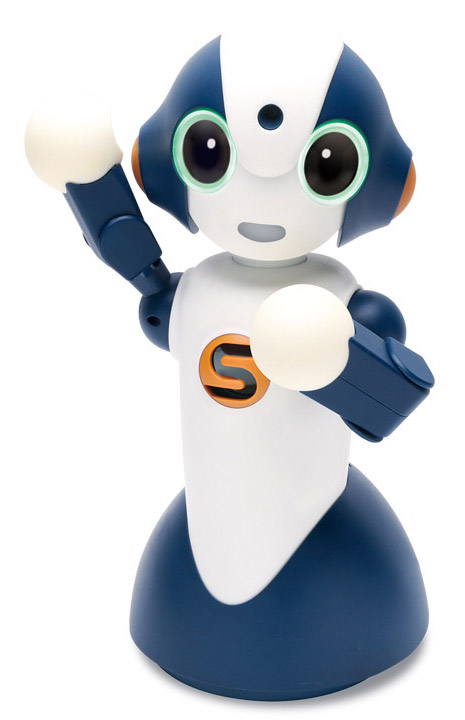
\includegraphics[width=\textwidth]{Thesis/data/sota.jpg}
		\caption{\centering Sota robot of NTT DATA }
		\label{fig:sota}
	\end{subfigure}
\caption{Example of humanoid robots}
\label{fig:humanoid}	
\end{figure}

\item Not human-like: in general are any robots with a body shape not inspired to the human body. But in the specific case of social robots, often these are inspired by animals as Miro the like-pet robot developed by Consequential Robotics showed in fig \ref{fig:miro}. 
In fact, one of the most common communications after that between human-human and that between human and humanoid robot is that with one's own pets in which even without verbal communication a non-verbal conversation can be established.
Obviously, however, the robot under consideration does not necessarily have to be inspired by an animal, it is enough that it has social skills able to  autonomously establish a communication with the user. An example of a social robot neither humanoid nor like-pet is Vector developed by Anki and shown in the fig \ref{fig:vector}.
\end{itemize}
\begin{figure}[H]
	\centering
	\begin{subfigure}{0.31\textwidth}
	    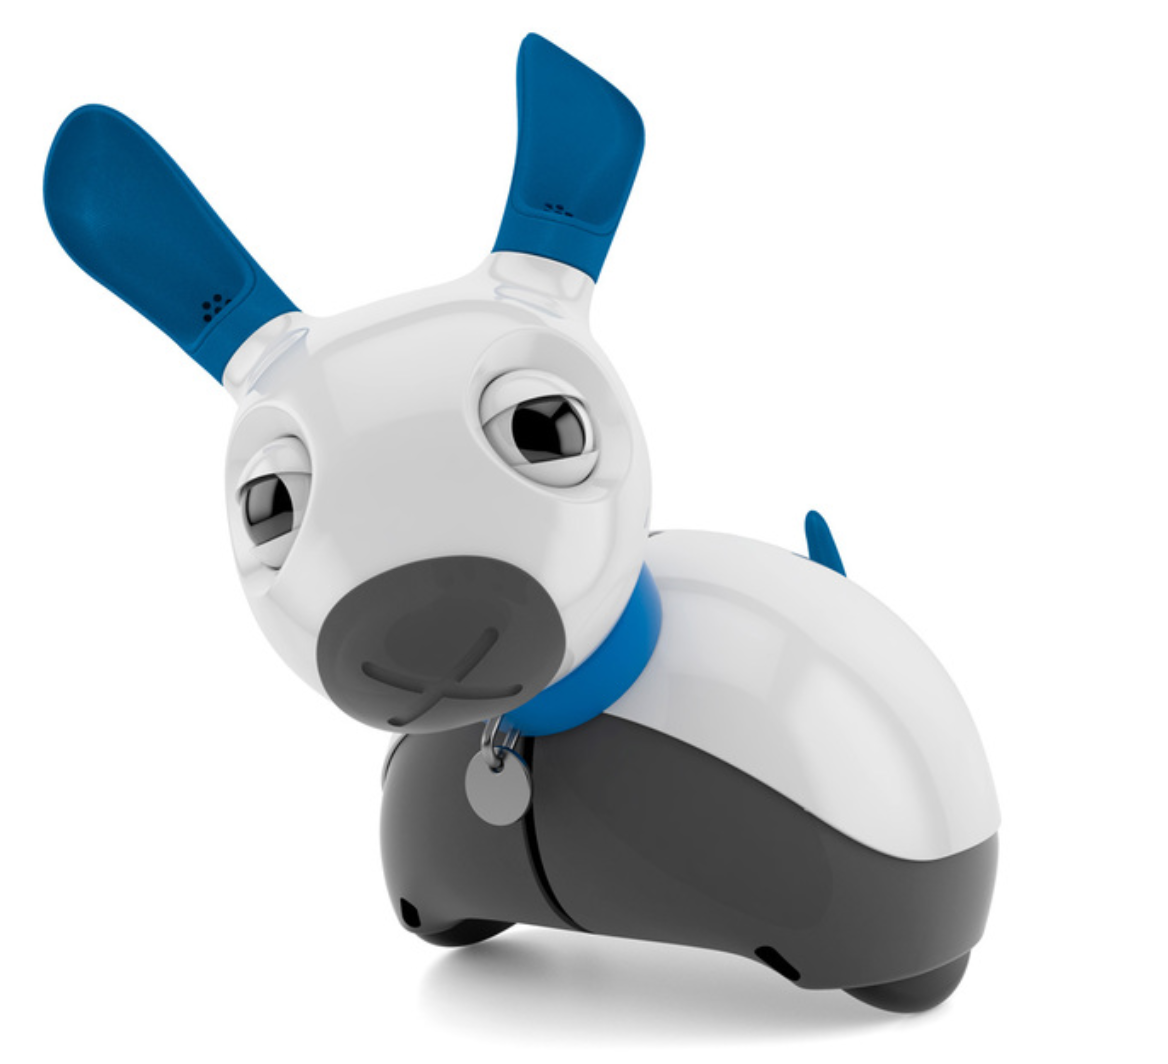
\includegraphics[width=\textwidth]{Thesis/data/miro.png}
         \caption{\centering Miro robot of Consequential Robotics}
        \label{fig:miro}
	\end{subfigure}
	\begin{subfigure}{0.31\textwidth}
		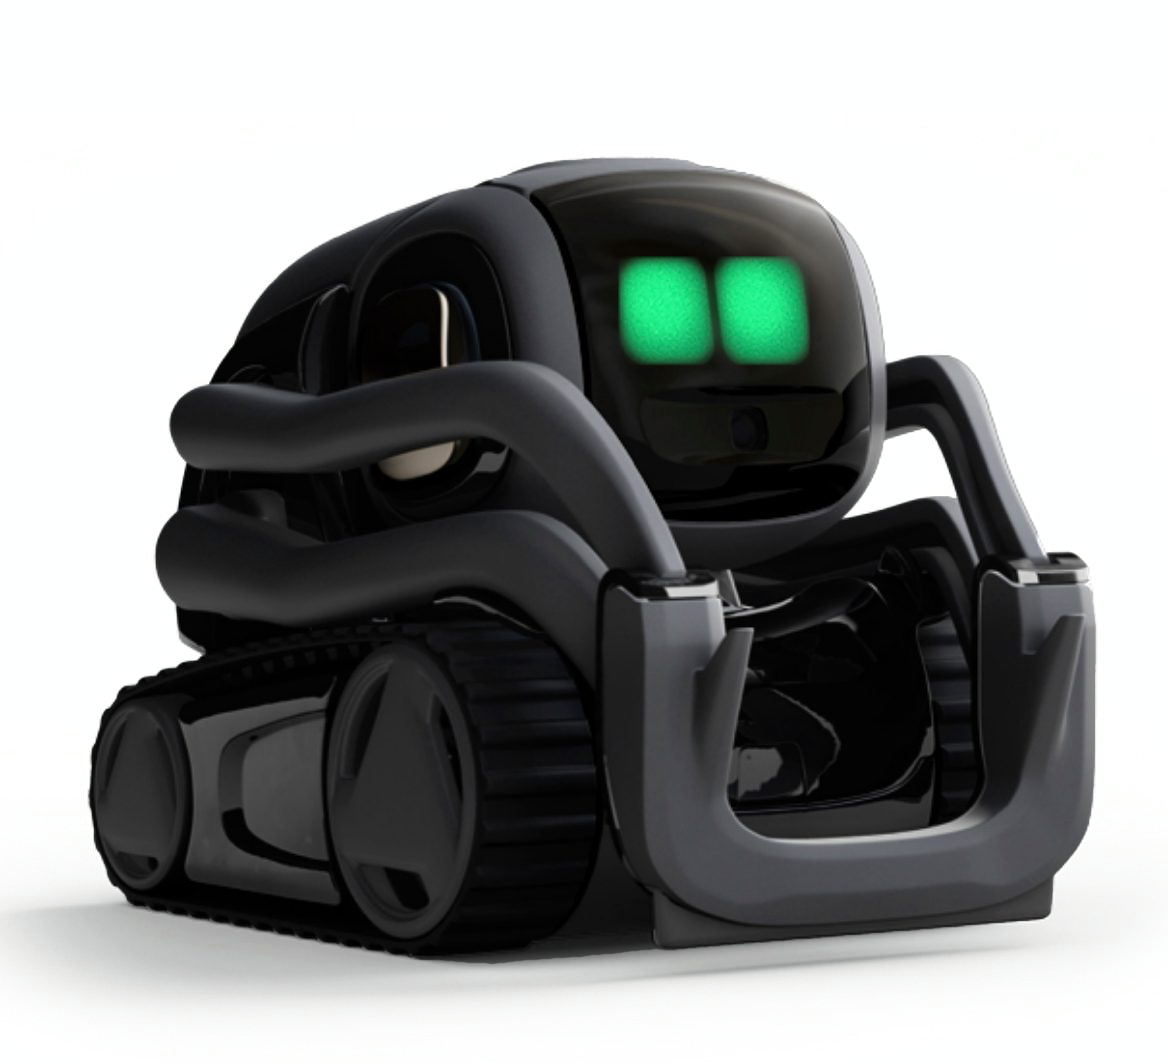
\includegraphics[width=\textwidth]{Thesis/data/vector.png}
		\caption{\centering Vector robot of Anki}
		\label{fig:vector}
	\end{subfigure}
\caption{Example of non-humanoid robots}
\label{fig:non-humanoid}	
\end{figure}

\subsection{Non-Embodied interface}
When the interaction is no longer bound to a physical body or more generally, it is completely unrelated to any physical limitation, we speak of non-embodied interface. These interfaces are typically auditory (with vocal interfaces), visual (with screens), tactile or combinations of these. On the one hand these kind of approaches allow a simpler and cheaper interface on the other are less “complete" from the point of view of social skills.


% \section{Human Activity Recognition}
% There are many papers in literature where are discussed the automatic recognition of ADL. There are often differences about adopted sensing equipment or in the choice of the type of sensors, but typically all the solution share a common paradigm: ``\textit{distributed sensing, centralized reasoning}". The sensor information are distributed as raw data, with minimal or no processing, and made available to the reasoning system responsible for analyzing them to extract high level information, the ADL \cite{buoncompagni2017towards}.   

% % A possible solution is to use binary sensors for their easy interpretation (eg: ON/OFF light switch) and their low cost. However, sensory information must be organized and analyzed in higher-level structures and this in literature, the most common and smart solution is doing it with \textit{ontologies}  already discussed in section \ref{ontology} \cite{buoncompagni2017towards}.

% \section{Recognition Reliability} \label{reliability}
% The reliability of the recognition is obviously fundamental for any system. Indeed we need to discriminate when a solution is consistent, when all the information is coherent or not with the specific activities detected, when there are some missing information or contradictory.
% Therefore along with the correct recognition of activities, a model should also be capable of detecting and avoiding false assignments \cite{iannello2009use}. Most of the activity recognition approaches while focusing on the segmentation and recognition may ignore false assignments \cite{rashidi2011discovering}. Additionally the existing approaches that exploit the temporal pattern for recognition assume that the activities follow a certain predefined sequence of events, however a fixed sequence may not always be the case, since a single activity can be performed in different ways by different users \cite{chikhaoui2012adr}.


 \chapter{State of the art}
 % ~~~~~~~~~~~~~~~~~~~~~~~~~~~~~~~~~~~~~~~~~~~~~~~~~~~~~~~~~~~~~~
% SOCIAL - COMPANION ROBOT
% Animal visits as emotional support ~ companion robot same advantages withouth take care -  “The psychosocial effects of a companion robot: a randomized controlled trial”

% Companion robot Paro improve mood - “Long-term robot therapy in a health service facility for the aged-a case study for 5 years”

 % Robot  with more social abilities = higher score on Perceived Enjoyment + higher Intention to Use the system- “The influence of social presence on acceptance of a companion robot by older people”

 % The enjoyment using a conversational robot bring influence acceptance of the tecnology - “Enjoyment intention to use and actual use of a conversational robot by elderly people”

 %  User acceptance and the users’ attitude towards the robot - “Evaluation of human robot interaction factors of a socially assistive robot together with older people”

 % Positive perception of the robot - “A Robot at Home ~ How Affect, Technology Commitment, and Personality Traits Influence User Experience in an Intelligent Robotics Apartment”

 % Psychological factors that promote acceptance or rejection of robots by older people  - “Does the Robot Have a Mind? Mind Perception and Attitudes Towards Robots Predict Use of an Eldercare Robot”

 % Matching between robot’s behaviour and it’s task = people acceptance - “Matching Robot Appearance and Behavior to Tasks to Improve Human-Robot Cooperation”

 % Effective human/robot interfaces which mimic how humans interact with one another could ultimately lead to robots be­ ing accepted - “Interactive Robot Task Training through Dialog and Demonstration”
 
 % ~~~~~~~~~~~~~~~~~~~~~~~~~~~~~~~~~~~~~~~~~~~~~~~~~~~~~~~~~~~~~~
 % VOCAL 
 % The UTAUT aims to explain user intentions to use an information system and subsequent usage behavior. The theory holds that there are four key constructs: 1) performance expectancy, 2) effort expectancy, 3) social influence, and 4) facilitating conditions - USER ACCEPTANCE OF INFORMATION TECHNOLOGY: TOWARD A UNIFIED VIEW

 % Voice interface = overall acceptance (for elderly) - “Design and evaluation of a smart home voice interface for the elderly: acceptability and objection aspects”

 % Non-embodied  vocal interface - “Improving Operational Support in Hospital Wards through Vocal Interfaces and Process-Awareness”
 

 % ~~~~~~~~~~~~~~~~~~~~~~~~~~~~~~~~~~~~~~~~~~~~~~~~~~~~~~~~~~~~~~
% Social ROBOT + VOCAL interface
% (a) create a positive bias in user’s perception of technology in the environment
% (b) increase user acceptance for the home dialogue system, and 
%(c) trigger social behaviors of the user towards the home dialogue system. - Benefits of Social Intelligence in Home Dialogue Systems

% conversational social robot results have indicated a high user satisfaction rate validating the robots capability to interact in a human-friendly manner during service assistance. - Design and Development of an Interactive Service Robot as a Conversational Companion for Elderly People

% Overview to accept Robot- Understanding Robot Acceptance

% Social intelligence = better communication, more comfortable, more acceptable - “Studying the acceptance of a robotic agent by elderly users”

% utility, usability, social acceptance = acceptance tecnology - “Acceptability in interaction - From robots to Embodied Conversational Agent”

% ~~~~~~~~~~~~~~~~~~~~~~~~~~~~~~~~~~~~~~~~~~~~~~~~~~~~~~~~~~~~~~
% GENERAL ACCEPTANCE
% Technology acceptance Model - “A technology acceptance model for empirically testing new end-user information systems: Theory and results” 

% ~~~~~~~~~~~~~~~~~~~~~~~~~~~~~~~~~~~~~~~~~~~~~~~~~~~~~~~~~~~~~~
% USER MODEL
% - A Robot at Home – How Affect, Technology Commitment, and Personality Traits Influence User Experience in an Intelligent Robotics Apartment
 
 
 \section{Arianna\texorpdfstring{$+$}{+}} \label{Arianna}    
 In this Section, the objective will be to describe a knowledge-based approach for domain modeling (i.e., context/activity modelling) and reasoning (i.e., context/activity recognition), which is currently part of Arianna$+$ smart home framework~\cite{kareem2018arianna}. \\
%  Arianna+ is widely described by two papers \textit{Towards a new paradigm for assistive technology at home} of \textit{Buoncompagni et al.} \cite{buoncompagni2017towards} and \textit{Arianna+: Scalable Human Activity Recognition by Reasoning with a Network of Ontologies} of \textit{Yusha Kareem et al.} \cite{kareem2018arianna} I'll therefore avoid citing them to allow for a better reading.\\
 Arianna+ is described by two papers \textit{Towards a new paradigm for assistive technology at home} \cite{buoncompagni2017towards} and \textit{Arianna+: Scalable Human Activity Recognition by Reasoning with a Network of Ontologies} \cite{kareem2018arianna}, wherein they show it's potential and features. This section mainly refers to them and outlines the key concepts within them. Domain modelling in Arianna+ is based on the following:
 \begin{itemize}
     \item Ontology Web Language (OWL), based on description logics (DL), allows to describe a given domain by defining relevant concepts (in the terminological box or TBox) and by asserting properties of individuals that are instances of those concepts (in the assertional box or ABox).
     Reasoners can then be used to derive facts, i.e., make implicit knowledge explicit, by reasoning mechanism \cite{donini1994deduction} based on \textit{subsumption} of concepts and \textit{instance checking}.
     \item Rules based on the Semantic Web Rule Language (SWRL) extend the OWL axioms. They provide high-level abstract syntax for Horn-like rules which are in the form of an implication between an antecedent (body) and consequent (head). The intended meaning can be read as: whenever the conditions specified in the antecedent hold, then the conditions specified in the consequent must also hold \cite{horrocks2004swrl}. For example, \\
     \texttt{Person(?p)} $\wedge$ \texttt{hasAge(?p,?age)} $\wedge$ \texttt{swrlb:greaterThan(?age,17)} $\rightarrow$ \texttt{Adult(?p)}.
 \end{itemize}
 
  OWL-DL reasoners are not able to perform temporal reasoning due to issues of language expressivity. Nevertheless it is possible to have within an ontology, temporal concepts by hooking onto an upper ontology called OWLTime that provides concepts related to Allen’s temporal algebra \cite{kareem2018arianna}. Nevertheless, a close-knit interaction between OWL-DL and an extra logic language (i.e., JAVA), enables temporal reasoning in Arianna+.
  
  In the literature, there have been attempts \cite{scalmato2013describing,buoncompagni2017towards} at ontology-based AR, that take temporal reasoning into account by accumulating temporal instances within the ontologies. Hence, their search space grows exponentially \cite{salguero2018using}, as the number of axioms grow within the ontology, which is an issue for real-time and large-scale applications. On the contrary in Arianna+, a close-knit interaction between OWL-DL and JAVA, allows temporal reasoning without accumulating temporal instances within the ontologies.

%  In a real-world environment, it is crucial that AR systems carefully guarantee \textit{scalability} and \textit{robustness} requirements \cite{kareem2018arianna}.
%  \begin{itemize}
%      \item The scalability can be achieved when the system is:
%      \begin{itemize}
%          \item modular with respect to the type of sensors, designing a system’s architecture that incorporates distributed sensors data;
%          \item modular with respect to the activity models, designing them modularly as part of an ontology network, which is able to infer activities based on the occurrence of events;
%          \item able to manage computational resources and memory, designing the activity models such that they represent the context over time, and evaluate them with the most suitable behaviour (e.g., with a scheduled frequency). Since they affect recognition performance in long-term applications 
%      \end{itemize}
%      \item The system’s robustness can be increased with redundancy of models with which we can assess the same activity;
%  \end{itemize}
 
In a real-world environment, it is crucial that AR systems carefully guarantee \textit{scalability} and \textit{robustness} requirements \cite{kareem2018arianna}.
The scalability can be achieved when the system is: (a) modular with respect to the type of sensors; (b) modular with respect to the activity models; (c) able to manage computational resources and memory. Arianna+ meets these constraints, by having a system's architecture that (a) incorporates distributed heterogeneous sensors; (b) has a network of ontologies in its reasoning layer, wherein each modular ontology is an activity model; (c) reasons based on particular ontologies, which are activated in the network based on context; rather than reasoning based on all the ontologies in all contexts.
Finally the robustness, is increased with redundancy of activity models, i.e., the same activity can be recognized with different activity models.

 \subsection{Activity Detection}
 \subsubsection{Dynamic Ontology Networks}
 In practice, Arianna+ corresponds to a network of ontologies tasked with performing a distributed reasoning process, each one dealing with different levels of detail in knowledge representation. 
 A fundamental step to reach this goal is  the definition of an activity model, its components and the procedures to evaluate it. In particular, Arianna+ describes each data sample through a generation time instant (T) and a fluent statement defined as a combination of a Boolean state (e.g., top $\top$ and bottom $\bot$).
 
 The recognition of an activity is represented as a new belief that acquires the Boolean $\top$ value by specifying the moment in which the execution of the activity is deduced.
 
 In this way, more complex models can be built as chains of sub-models, since their outcomes are statements, which can be embedded in more complex statements.
 This makes the Arianna+ reasoning engine scalable and suitable for asserting same activity in different.
 
Morover Arianna+ allows the use of simpler concepts to recognize several more complex concepts sharing the beliefs  with other models. For example, once the activity has been recognized as \textit{``cabinet door opened"}, it can be used to recognize an activity such as \textit{``leaving an object"} or \textit{``taking an object"} and both can be used to conclude that the person is \textit{``cooking"}.

 In Arianna+ statements are grounded in a DL-based formalization. A \emph{Statement} is defined as a concept whose instances are restricted to have, exactly one property specifying the state of the statement and exactly one property specifying the time instant of the statement's generation.
 
 \begin{equation}
     X : Statement \doteq \exists_{=1} hasState(X, s_X) \sqcap \exists_{=1} hasTime(X, t_X)
     \label{statment}
 \end{equation}
 
 The ontology network is defined as a graph $G$, wherein the set of nodes $N$ are ontologies (each with an independent DL reasoner) containing statements of the form \ref{statment} and they are used to describe a specific part of the context, while the set of directed edges E are communication channels used for sharing statements between the nodes.
 
 Hence $G$ is of the form:
 \begin{equation}
     G = \left \{ N, E \right \}
 \end{equation}
 where, $N = n_1, n_2, ... , n_n$, so that each $node$ specializes in reasoning within a particular context, and $ E = e_{12},e_{13},...,e_{1n},e_{21},e_{23},...,e_{2n},...,e_{mn}$, so that the index of each $edge$ signifies the direction of flow of statements, e.g., in $e_{12}$ statements flow from $n_1$ to $n_2$. 
 
 The system checks the statements in the network with a given frequency and, when an event is detected, specific external procedures are executed in order to: (i) move statements from one node to another via edges, and (ii) evaluate models for activity recognition. For instance, statements could be generated from distributed sensors (e.g., detecting that Adam is in the kitchen at 8:00 am) and then the system aggregates this information with prior knowledge to detect events (e.g., Adam is in the kitchen in the morning). When such an event occurs, the model used for detecting that Adam is having breakfast is evaluated by checking statements and their temporal relations within the model.
 Moreover, activity models can generate statements, e.g., indicating that Adam had (or did not have) breakfast at a certain time, and hence can trigger new events, which can further be used to describe the context and evaluate models via procedure executions. A formal algebra of statements, used for defining events that execute procedures based on the context, has been proposed by \textit{Buoncompagni et al.} \cite{buoncompagni2017towards}.
 
 \subsubsection{A Network of Activity Detectors}
 To better understand the system let's try to consider a simplified ontology network $O$ as shown in \ref{fig:simplifiedOntologyNetwork}.
 Inside there are six nodes $n_i$ for $i=1,..,6$ where:
 \begin{itemize}
    \item $n_1$ is a location-based contextualizing model called \textit{Place Ontology P};
    \item $n_2,...,n_6$ correspond to \textit{activity models} and can be called $A_j$ for $j=1,...,5$;
 \end{itemize}
 
 Among these nodes we can therefore distinguish two types of statements where:
 \begin{itemize}
     \item within $P$ only the spatial aspect is taken into account;
     \item within each $A_i$, both spatial and temporal aspects are taken into account;
 \end{itemize}
 
  \begin{figure}[h]
	\centering
	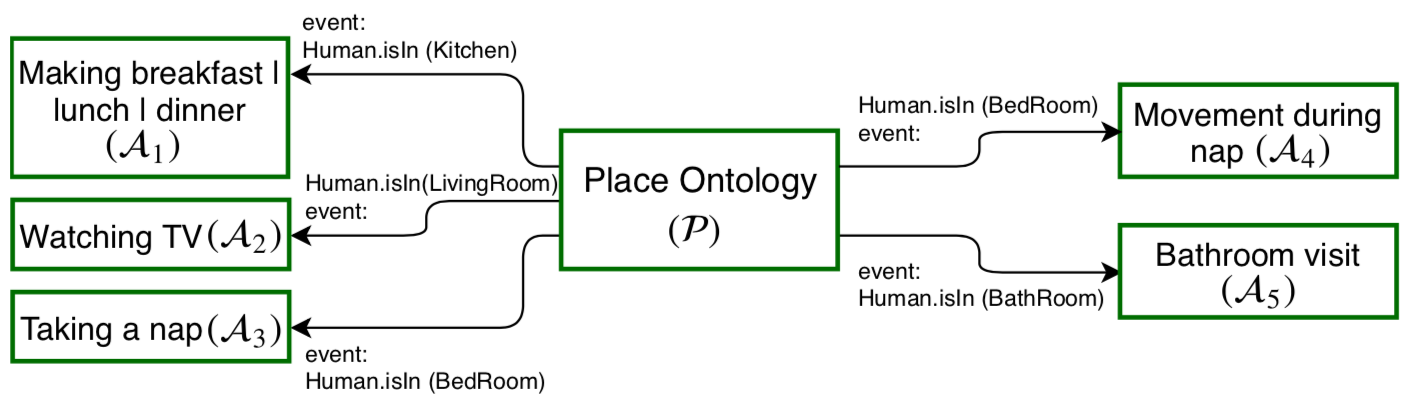
\includegraphics[width=15cm]{Thesis/data/O.png}
	\caption{A simplified ontology network $O$ \cite{kareem2018arianna}.}
	\label{fig:simplifiedOntologyNetwork}
  \end{figure}
   \begin{figure}[H]
	\centering
	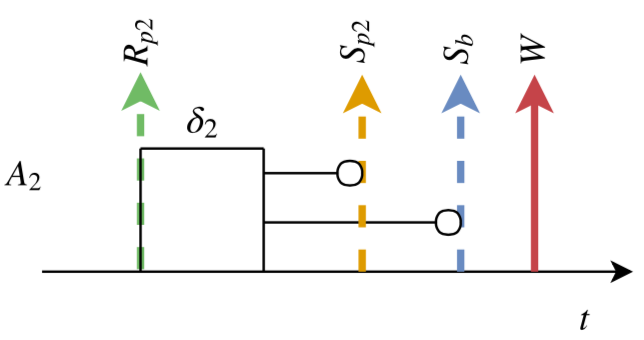
\includegraphics[width=8cm]{Thesis/data/event.png}
	\caption{``Visual representation of statements that make up the A2 model: statements are shown as vertical arrows where dashed arrows indicate information from $P$, and solid arrows indicate statements generated by this model. Statement indexes indicate sensors influencing the state of that statement, while the temporal restrictions are shown as black lines \cite{kareem2018arianna}."}
	\label{fig:A2}
 \end{figure}

 The internal mechanism between the nodes is as follows: the activity models $A_i$ constantly wait for $P$ to generate particular events, once an event is generated, for example \texttt{isIn(User, LivingRoom).\{hasState(True), hasTime(19:26)\}}), a particular activity is activated as shown in figure \ref{fig:simplifiedOntologyNetwork}, for example $A_2$ gets activated based on the above exapmple. As we can see in the figure, statements flow between nodes through the edges $E = e_{12}, e_{13}, e_{14}, e_{15}, e_{16}$. Furthermore, a procedure related to an activity model, generates a new statement to notify the recognition of an activity when the model gets satisfied, for example in case $A_2$ gets satisfied, the following statement gets \emph{generated}, \texttt{WatchingTV.\{hasState(True), hasTime(19:28)\}}.
 
    % \begin{algorithm}
    % \caption{Internal mechanisms between the nodes}\label{alg:euclid}
    % \begin{algorithmic}[1]
    % \Procedure{communication between nodes}{}
    % \State $A_i$ constantly wait for $P$ to generate particular events;
    % \State Statements are shared between nodes through the edges $E = e_{12}, e_{13}, e_{14}, e_{15}, e_{16}$;
    % \State Instructions flow between the various nodes through the edges;
    % \State Activities are activated when their independent reasoners check an event as shown in figure \ref{fig:simplifiedOntologyNetwork};
    % \State A procedure generates a new declaration to notify the recognition of the activity when a model is satisfied;
    % \EndProcedure
    % \end{algorithmic}
    % \end{algorithm}
     
 To make sure that an activity has been recognized correctly, certain statements and temporal relationships must be satisfied.
 
 Figure \ref{fig:A2} graphically depicts A2 activity model ``watching TV", where: the arrows pointing upwards indicate a true state, the arrows pointing down indicate a false state, the dashed arrows represent instructions from another node, in this case from $P$ and finally, the solid arrows are generated by their own node, i.e., in this case by $A_2$.
 
 ``In the Figure \ref{fig:A2}, we can see 4 statements: (i) statement $R_{p2}$, which is a dashed arrow of green color, is information coming from $P$; it signifies \texttt{isIn LivingRoom.{hasState(True), hasTime(19:25)}}, where the index $p2$ indicates that the sensor \texttt{PIR2} influences the state of this statement; (ii) statement $S_{p2}$, which is a dashed arrow of orange color, is information coming from $P$; it signifies that there is some motion in the living room after $\delta_2$ time units, naively representing the idea that, if Adam is sitting on the sofa then he is not sitting still; this statement can be replaced by a much robust statement, for instance, \texttt{sitting.{hasState(True), hasTime(19:26)}}, given that there may be other sensors in the system (e.g., wearable sensors, pressure sensors in the sofa); (iii) statement $S_b$, which is a dashed arrow of blue color, is information coming from $P$; it signifies \texttt{highBrightnessTV.{hasState(True), hasTime(19:28)}}, where the indexes $b$ indicates that brightness sensor influences the state of this statement; (iv) statement $W$, which is a solid arrow of red color, generated once the overall model is satisfied, it signifies \texttt{WatchingTV.{hasState(True), hasTime(19:28)}}; this happens when statements $S_{p2}$ and $S_b$ are generated after $\delta_2$ time units with respect to the $R_{p2}$ statement \cite{kareem2018arianna}".
 

 It is important to note that when $A_i$ receives instructions from $P$, the values of the older instances get updated (if they are available), performing temporal reasoning using both symbolic relations (inferred by the DL reasoner) and numerical/logical operations on the timestamps (inferred externally). 
 After an activity is recognized, the statements are removed to reduce disk usage and the increasing complexity of the ontologies. 
 
%  \subsection{Recognition Reliability}
%  %As explained in Section \ref{reliability} of the first Chapter, it is important to perform consistency checks to describe the context as a semantic hierarchy to be applied to statements over time.
%  The reliability of the recognition is obviously fundamental for any system. Indeed we need to discriminate when a solution is consistent, when all the information is coherent or not with the specific activities detected, when there are some missing information or contradictory.
%  It is important to perform consistency checks to describe the context as a semantic hierarchy to be applied to statements over time.
 
%  To do this Arianna+ uses the specifications of OWL API and Pellet \cite{buoncompagni2017towards} to define semantic classes (indicated using capitalized names) and properties in their definitions (indicated with be/have characteristics), in order to allow the reasoner to classify individuals based on facts that have to be held true (in consistency terms) in the description of the environment.
 
 \subsection{Arianna+’s Architecture}
 In the Arianna+'s architecture we can distinguish sensing, aggregation, reasoning and application layer.  
 The ontology network $O$ is used over time to recognize activities based on the data taken from the database ($DB$), which stores the last values and timestamps coming from the aggregation layer which itself takes the data from the physical sensory layer.
 All the $DB$'s information are taken by the application layer to provide to the user a GUI to interact with.  
 
 \begin{figure}[ht]
	\centering
	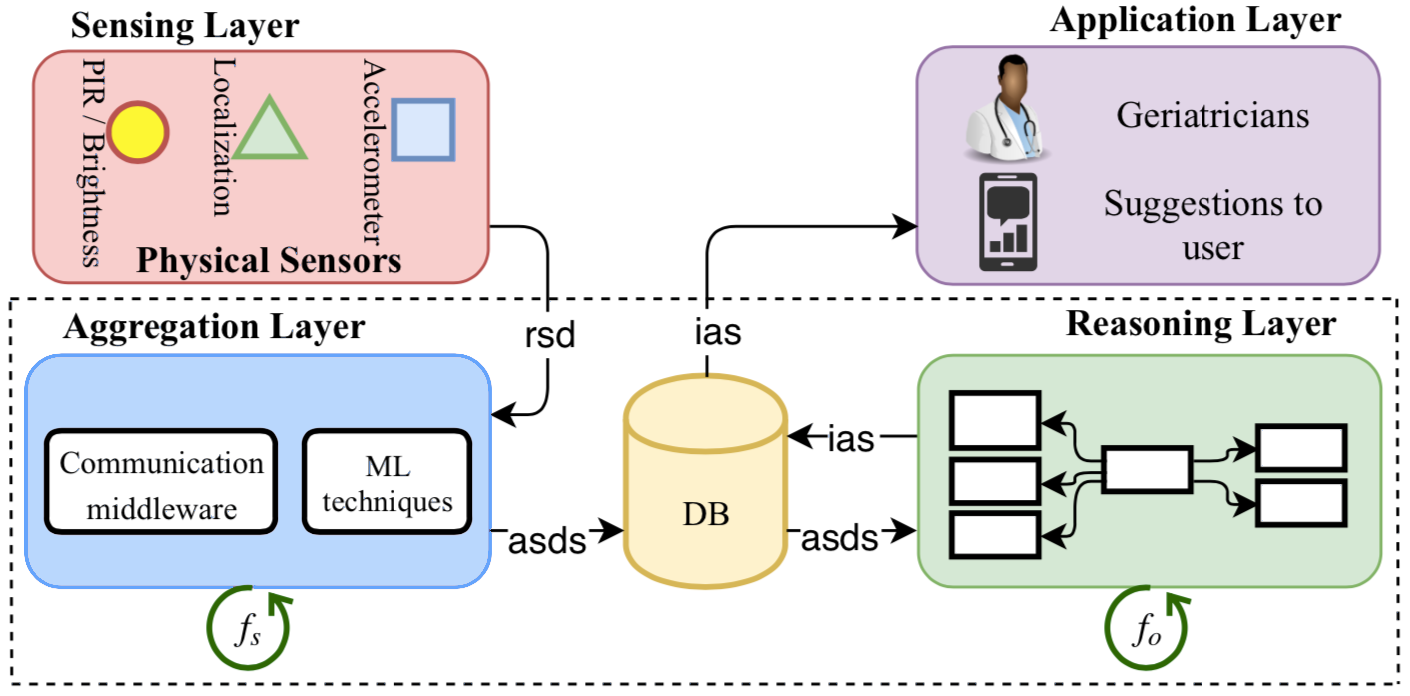
\includegraphics[width=17cm]{Thesis/data/layers.pdf}
	\caption{``Arianna+ ’s architecture where the link rsd signifies the flow of raw sensor data, \textit{asds} signifies the flow of aggregated sensor data in the form of statements, \textit{ias} signifies inferred activity statements and f signifies frequency. \cite{kareem2018arianna}"}
	\label{fig:layers}
 \end{figure}
 
 Now let's consider the tasks that the individual layers play:
 \begin{itemize}
     \item The \textit{reasoning layer} can be considered the core of Arianna+ in fact it corresponds to the ontology network where it is possible to distinguish two components:
     \begin{enumerate}
         \item initialization of the ontology network $O$ where the procedures and events are defined as edges and the TBox ontologies are defined as nodes;
         \item reasoning with a frequency $f_o$. Wherein, the procedure associated to $P$: takes the aggregated sensors data from the database (i.e., link asds), updates the ABox in $P$, reasons (spatially) with the knowledge acquired in $P$ and declares an event if there is one.
     \end{enumerate}
     Hence the event can activate the procedures of one or more activity models $A_i$. The procedures then update ABox of the model they are associated to and on the basis of the new knowledge within the model, reasoning (spatially and temporally) is done and finally if an activity truly happens, it gets recognized.
     
     
     So if an activity is recognized, the procedure associated with the model saves the statement of the derived activity (link ias) in the database and if the update of the information corresponds to an event it can restart the process.
     
     Unfortunately, the time computation of the reasoning process is not negligible so if the frequency with which new data arrives is faster than the reasoning, the system would not meet the near real-time constraint.
     For this reason we have to face the problem of the computational complexity of the DL reasoner by inserting a control system that manages the processes of reasoning based on their computational complexity.
     
    \item The \textit{application layer} is developed for two types of users:
    \begin{enumerate}
        \item for the geriatrician who can view statistics on the activities performed and explore further details such as vital signs and sleep quality;
        \item for the elderly person who could visualize suggestions based on his activities interfacing for instance through dialogue-based interfaces via virtual coaches;
    \end{enumerate}
    In addition, the database keeps track of $O$ statements so that medical or assistive staff can use or view them to provide additional services to the elderly.
    \item The \textit{aggregation layer} takes the raw sensors data from the detection level (link rsd), processes the raw data to generate statements in the format specified at (\ref{statment}) to store them in the database (link asds). This level can therefore be considered an intermediary level of processing of the raw data, which is based on classification modules (e.g., machine learning approaches) that allow to directly provide statements with semantics (e.g., sitting down).
    
    Moreover it is important to note that a statement with formal structure allows not only a modular approach to the evaluation of activities but also allows the system to take information from heterogeneous sensors. The whole process of elaboration can be more or less expensive from the point of view of computational time, for this reason according to the statement, not only it must consider the frequency with which the level of aggregation saves the information of the database but also the computational time required for the single module to aggregate the information.
 \end{itemize}
 
  The aggregation and reasoning layers are connected through the database where all the statements are stored, this is a means of communication between the two layers thus allowing $2$ different layers to work at different frequencies. In fact, the aggregation layer stores the aggregated statements and updated them with a frequency $f_s$ while the reasoning layer bases its reasoning on the updated statements present in the $DB$ and taken every $\frac{1}{f_o}$ seconds.
 
 \section{Companion Robot}  \label{companionRobot}
 
 Most often for the elderly, moving to a retirement home is often caused by the loss of someone close or by the inability to look after himself due to the decline of his health or lack of control over his life.
 This means that the elderly at this stage of life loses certain aspects of their life that make them independent and satisfied.
 
 In fact, in nursing homes especially in the first phase of the stay, the elderly feel isolated, impotent and bored with the consequent risk of depression and loneliness.
 Unfortunately, even when they get used to staying in a nursing home, the feelings of loneliness and the isolation do not disappear because they are left with difficulty of establish new relationships \cite{assistiveRobots}.
 
 In the past, for an emotional support, many care homes incorporated animal visits, because they help fulfill criteria aimed at promoting better quality of life for the elderly by \cite{psicologicalEffects}: helping to create social relationships and hence increasing the social interactions, decreasing loneliness, countering boredom and helping foster a sense of purpose. 
 
 Moreover, almost anyone, despite their physical and cognitive damage, could interact with an animal.  \\
 In fact, interactions with animals have three effects \cite{psicologicalEffects}: (i) physiological effect (e.g. improvement of vital signs), (ii) psychological effect (e.g. improvement of mood and depression), (iii) social effect (e.g. facilitates communication).

 The success of the animal is a fact, however unfortunately an animal needs care, and care staff of a nursing home must already take care of the elderly, therefore they often do not have the desire or time to take extra care of an animal.
 A robot companion on the other hand can have the same advantages as a real animal, yet no care or attention must be given to it because it is autonomous \cite{psicologicalEffects}.
 In fact, the companion robots do not scratch or bite and don't host parasites or infectious diseases.
 
 In a study made in Japan, 14 residents who suffered from mild to moderate dementia were given the robot companion Paro \cite{wada2009long}. The results yielded an improvement in mood and depression and reduced stress levels; 
 The support staff defined the robot as a necessity because it made the elderly laugh and become more active by strengthening social ties.
 Unfortunately, studies like these are not solid because they generally take place within small samples and for a short period of time \cite{psicologicalEffects}.
 
 We can distinguish different assistive robots categories (fig: \ref{fig:typeRobot}) \cite{assistiveRobots}:
 \begin{itemize}
     \item \textit{rehabilitation robots} that help patients rehabilitate physical disabilities
     \item \textit{assisitive social robots} which are of two types. On one hand are \emph{service type} which are not perceived as a social but rather as a supportive. In fact, they help the elderly to remain with or regain their, independence in the functions of their every day and simultaneously allow the monitoring of their functions. (e.g.: artificial limbs). On the other hand, there are \emph{companion type} which aim to provide health and psychological well-being of elderly users by keeping them company. For this type of robotic solution, the expressiveness of emotions during the interaction with the human is crucial.
 \end{itemize}
 
 \begin{figure}[ht]
	\centering
	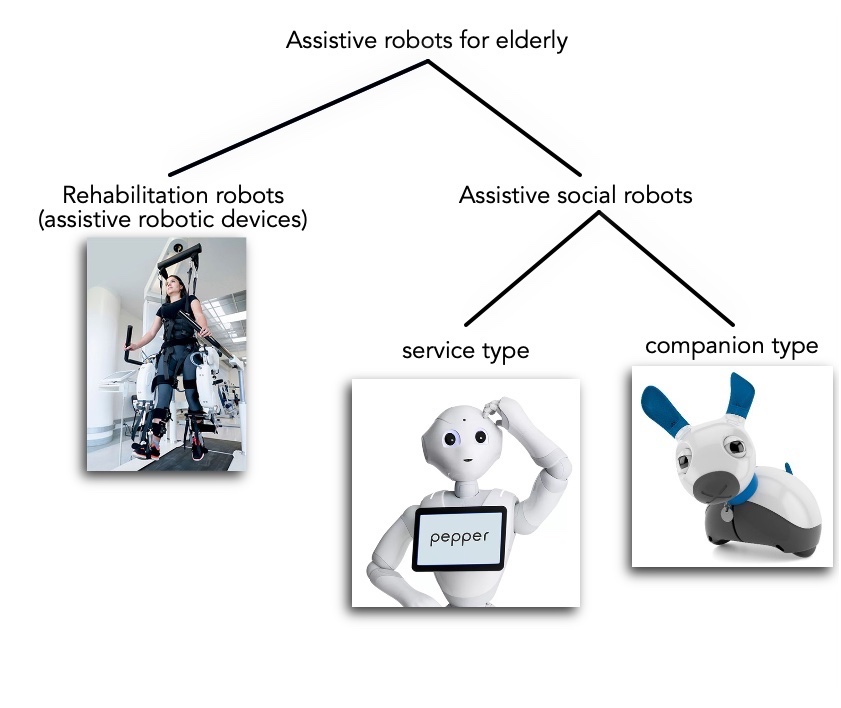
\includegraphics[width=14cm]{Thesis/data/TypeRobot.jpg}
	\caption{``Categories of assistive robots for elderly" \cite{assistiveRobots}}
	\label{fig:typeRobot}
 \end{figure}
 
 In assistive domotic, the distinction between assistance and companion robots is thin and often superfluous because it is possible to combine the characteristics of both types in a single robotic solution. In fact, the robotic technology in eldcare hardly develops just to entertain.
 For example, a robot could be able to monitor the status of the elderly and keep them company helping to interact with other people and with technology.
 
 It is noteworthy that the use of a robot companion positively influences the acceptance of technology by the elderly and this is crucial if you want to move the elderly into a smart home.
 
 In fact, the user considers the robot as a piece of technology with more or less easy to accept personality.
 Numerous studies have been done to ensure that above all, the elderly user is accepting of the technology \cite{heerink2008influence, enjoymentModels,assistiveRobots}.
 
 In technology acceptance models, enjoyment is sometimes incorporated as ``Perceptual Enjoyment" which is defined as: "the extent to which the use of the system is perceived as enjoyable in itself, regardless of the consequences on performance that may be anticipated" \cite{enjoymentModels, davis1992extrinsic}.
 
 In general, the acceptance of robots or intelligent agents takes place in terms of \emph{functional acceptance}, i.e., usefulness and ease of use, and \emph{social acceptance} where a Robot-Human relationship is established, with a robot as  a conversational partner.
 
 The first concept of a model of acceptance dates back to 1986 "Technology Acceptance Model for Empirically Testing New End-user Information Systems Theory and Results" which is still now the theoretical model among the most used in behavioral psychology \cite{davis1985technology,enjoymentModels}.
 It states, in its most basic form, that ease of use and perceived usefulness determine the behavioral intention of using a system.
 
 In 2003, \textit{Venkatesh et al.} published an inventory of all current models and factors and presented a new model called UTAUT \cite{venkatesh2003user,enjoymentModels} which covers the constructs of, performance expectation, effort expectation, aptitude for the use of technology, self-efficacy and anxiety.
 
 As previously discussed, when it comes to accepting robots, it is important not only to consider acceptance in terms of ease of use and utility of a system, but also of relational or social acceptance. This means that a user accepts the robot as a conversational partner finding credible social skills in the robot, considering the robot as an autonomous social being. 
 
 From this we can conclude that integration of a vocal interface along with a conversational partner, becomes crucial for the technological acceptance by the elderly. This topic is further elaborated in the section \ref{speech}.
 
%  In conclusion, we can summarize the advantages of using a robot companion in a smart nursing home:
%  \begin{itemize}
%      \item improves the health and psychological well-being of the elderly
%      \item does not need treatment unlike a real animal
%      \item can be used to monitor the elderly activities (in our case by integration with Arianna+)
%  \end{itemize} 
%  We hypothesize that these advantages enable technology acceptance by the elderly.
In conclusion, we summarize the advantages of using a companion robot in a smart nursing home, it (i) improves the health and psychological well-being of the elderly,(ii) does not need treatment unlike a real animal, (ii) can be used to monitor the elderly activities (in our case by integration with Arianna+) and (iv) can motivate the elderly to accept such technology.

 \section{Dialogue management system} \label{speech}
 \subsection{Fields of study}
 The traditional telephone and video conference systems are examples of iterations focused on the terminal, in which the user focuses his attention and gaze, fixed on the terminal. So when deciding to start and then to end a call, we turn on or off our attention directed at the terminal. This type of iteration has more or less the same social characteristics as a formal face-to-face meeting \cite{augusto2010ambient}.
 Likewise in an environmental communication, as a person could dialogue with another person in another room, the same the dialogue management system can interact with the  user .
 
 The study of the interaction between human and technology in smart environments is studied by two complementary research sectors:
 \begin{itemize}
    \item the Human-Robot Interaction (HRI) which can be defined as ``the study of humans, robots and the ways in which they influence each other". As a discipline, HRI concerns the analysis, design, modeling, implementation and evaluation of robots for human use.
    HRI is strongly related to Human-Computer Interaction (HCI) and Human-Machine Interaction (HMI). HRI, however, differs from HCI and HMI because it concerns systems (i.e. robots) that have more complex and dynamic control systems.
     
    \item social intelligence which, in its widest definition, is a person's ability to ``\dots get along with people in general, social technique or ease in society, knowledge of social matters, susceptibility to stimuli from other members of a group, as well as insight into the temporary moods of underlying personality traits of strangers." \cite{vernon1933some}.
 \end{itemize}

 Both play an important role because they both study how much and with which dynamics man relates to the technological system, from the point of view of design and engineering in HRI and from the psychological point of view in social intelligence.

 \subsection{Approaches and advantages}
%  There seem to be two views and probably complementary opinions about how humans interact:
%  \begin{itemize}
%      \item through a multitude of specific IT applications for each activity;
%      \item through a centralized user interface which anticipates the needs of users through the adaptability of intelligence;
%  \end{itemize}

There seem to be two views and probably complementary opinions about how humans interact. On the one hand, through a \emph{multitude} of specific IT applications for each activity on the other hand through a \emph{centralized} user interface which anticipates the needs of users through the adaptability of intelligence.

 In the home domain, dialogue systems shall be required to appear as intermediaries between the systems embedded in the home and the people within them.
 In general, people in smart environments would like to be monitored as little as possible. Especially for the elderly it is necessary a trade-off between benefits and the intrusion into privacy. In fact, \textit{Portet et al.} have shown that the degree of acceptance of intrusive technology varies according to the severity of their disease \cite{portet2013design}. 
 Furthermore \textit{Saini et al.} demonstrated that providing a domestic dialogue system with social intelligence and behaviours ensures that the system is perceived as socially intelligent, leading to a more positive experience for users, who will be encouraged not only to accept the dialogue system but also the embedded technology \cite{saini2005benefits}.
 
 The advantages of a good interface are clear and well documented in the literature.
 For example, in a study conducted by \textit{Portet et al.} many opinions were collected concerning the appreciation of vocal interfaces in care homes for the elderly. In fact, 95\% of users would have continued to use this system even if it did not work perfectly and therefore occasionally made some mistakes \cite{portet2013design}.
 However, another important result emerging from these studies is that regardless of the technology used, no smart home application will be successful if it does not fit the individual user.
 In fact without an adequate assessment of the needs of the assisted person, the design of an interaction system, for the integration of new technologies, could be vain.
 
 So a system for human-machine and machine-human interaction, as a dialogue management system, must allow the user to interact as naturally as possible. For that to happen it is necessary that the dialogue system not only correctly interprets the user's voice but also takes into account the context in which the user speaks.
 
 In the case of integration (i.e., of dialogue management system) with Arianna+. The overall system must be aware of the context in which the user exists. For example, consider the situation where, Arianna+ knows that the person is in the kitchen, the stove is turned on and it is 8:15pm; then it concludes that the user is cooking. In this situation, the new overall system should be able to interact and adapt its interaction based on the situation.
 %Therefore any Arianna+ requests or intervention will be able to take account of context
%  To obtain such a result, the system must able to adapt itself not only on the basis of the context but also of the  different operators with which it must, according to needs, communicate, adjusting its language and behavior.

 \subsection{Dialogue}
 By definition, dialogue is a communication process between two or more parts which requires sharing of context information. The style and the form of the dialogue can therefore vary according to the interlocutors and the context in which they are. In the same way, as a dialogue between a group of scientists in a laboratory is not the same of dialogue between teacher and her young student.
 However over the years it has been possible to determine many properties of dialogue are common to all.
 All the verbal communications between man and machine, computer or robot are made through an interface that according to Lansdale and Ormerod \cite{mccourt1996understanding} is controlled by 5 factors:

 \begin{itemize}
     \item \textit{linguistic competence} that is the ability to construct intelligible sentences and to understand the interlocutor speech. The dialogue between man and machine requires a vocabulary able to associate concepts with words or groups of these (eg: command words) and sequences of actions (grammar);
     \item \textit{conversational competence} is a crucial skill for any successful conversation. Unfortunately for the machine mechanisms like inference are much more complicated to adopt than to a person, who uses them without even noticing it. These, like other mechanisms, facilitate dialogue between people rather than a slower dialogue between man and machine. For this reason the user interface must be designed in such a way that users can unambiguously impart intentions and receive feedback;
     \item \textit{nonverbal skills} correspond to all those aspects of communication that concern the language of the body, in other words those gestures that add coherence to the dialogue. They act as adaptations and cues of control, providing information often redundant for a simpler and immediate understanding of the concept that one wants to express;
     \item \textit{medium constraints} correspond to the communication constraints imposed to the user to establish a dialogue, thereby implacably influencing the nature of the dialogue;
     \item \textit{task constraints} influence the structure of dialogue. In fact the lexicon as well as the structure of the language  varies depending on the context in which we are, to avoid misunderstandings and communicate complex information. In the same way as a military communication  will have a lexicon and a grammar completely different from a discussion between two people at the bar;
     
 \end{itemize}
 A factor not mentioned here but equally important is the experience. In fact, studies of experts have shown how the ability to assimilate and process information depends largely on the knowledge that you have of the topic. This is because the previous knowledge allows the experts to categorize and enclose more information in a single concept that instead may seem incomprehensible to a novice \cite{fong2001collaboration}.
 When a doctor starts a dialogue with a patient. The doctor initially takes control of the conversation, leading the dialogue to a sequence of questions and replies. On the other hand, when both interlocutors are experts in a specific subject matter, control of the conversation is shared by both parties.
 This dichotomy is presented in the same way in the user's interface which (1) guarantee to experts greater control than to novices (2) or ensure that the procedures, which the user is not able to do, are executed.

 \subsection{Dialogue management}
 Unless the interaction is basic, with a fixed and limited grammar, the human-machine interface systems require dialogue management.
 The simplest function of dialogue management is to translate user requests so that the computer can understand it. An example is LUIS \cite{williams2015fast}, a service offered by Microsoft based on machine learning techniques in which the machine is taught to interpret a voice input in a specific domain defining a priori a certain number of Entities and Actions. For example, with a voice input, ``go to the kitchen" could return such as \texttt{"Entity"=kitchen} and \texttt{"Action"=move}, which information could be easily interpreted by the machine as part of its knowledge domain.
 In addition, however, the system must be able to manage the change of role that can take place at any stage of the dialogue. Dialogue management systems can allow the user, or computer, to take the initiative depending on the case. The difficulty lies in fact in dialogues where the initiative can be taken during any phase of the dialogue \cite{churcher1997dialogue}.

 There are two common methods for managing a dialogue. On one hand there are \emph{graphs}, wherein the dialogue consists of a series of nodes connected to each other where the user can choose which ``to explore" (ex: ``for reservations, press 2"). In this way the possibilities of choice are limited and therefore also the error. on the other hand are \emph{frames}, wherein database queries drive the dialogue ensuring less robustness compared to graphs but at the same time allowing greater flexibility for role switching.
 
 \subsection{User Model}
 Since dialogue should be studied on the basis of the interlocutor, it is important to define a model of them, so there is a reasonable mutual understanding. For example, the information presented (e.g., text, graphics), collections (eg: filtered, classic) can be adapted for the user. A profile or model of the user containing a set of information describing him. This information can therefore be used by the dialogue manager because typically a dialogue is strongly dependent on the properties of the interlocutor (eg: level of knowledge or skills, personal preferences, reactivity, etc) \cite{fong2001collaboration}.
 Many of these properties can be attributed, for example, to social aspects, such as the place where they live. If for example the user is Japanese, they will have different customs from an American, together with different habits and different priorities. An efficient way to proceed is to define a generalization model, asking a small but targeted amount of information to the user. This makes it possible to define a generalized and stereotyped model that identifies the person within a sub-group properties that may be modified and added in successive phases \cite{fong2001collaboration}.

 \chapter{Conclusion}
 
 The goal of this literature review, was to understand the main concepts and technologies that aim to support the elderly.
 First, an investigation was carried out to explore the main issues and concepts that govern ambient intelligence field.
 The most common techniques for modeling and determining a context have been defined showing their strengths and weaknesses. Based on the review, we are inclined to adopt an ontology-based approach, due to its advantages for our application.
 The review also attempts to express the importance of detecting ADL, which are fundamental activities of daily living, that allow geriatricians to guage an elderly individual's level of independence.
 
 The field of research is vast, but above all there are a number of different technologies that are necessary to make this type of a project, adaptable and physically feasible within a real nursing home. 
 For this reason, we decided to choose an existing architecture, i.e., Arianna+, which aims to solve most of the problems listed above.
 %This allowed me to focus on my real goals:
%  \begin{itemize}
%      \item Give voice to our home so that it can not only be consulted, but capable of acting, addressing directly to the assisted, in which case a situation is ambiguous in the eyes of the reasoning system.
%      A vocal interface, however, is not only useful for this fact, as widely discussed in the section \ref{speech}, it helps the elderly to accept the technological environment that surrounds it, allowing a simpler interaction.
%      \item Inserting a robot companion in the home environment, as discussed in section \ref{companionRobot}, would improve the health and psychological well-being of the elderly by also helping them to accept the technology that surrounds and monitors them. Specifically, its use is essential to provide eyes to the home, making this invasion of privacy as acceptable as possible.
%  \end{itemize}

Therefore the goal of my thesis would be twofold. 
Firstly, to explore and analyze the advantages of integrating a vocal interface in a nursing home via Arianna+. We expect that, this integration would not only help the elderly with acceptance of technology but would also allow Arianna+ to seek clarifications in ambiguous situations by simply asking for the clarifications from the elderly. 
Secondly, to understand and provide; what would be, a friendly interface between the smart home and the elderly individual. In this regard, as discussed in section~\ref{companionRobot}, the use of a companion robot within a smart nursing home seems promising. As it not only has the potential for positive impact on the health and psychological well-being of the elderly individuals but would also enable Arianna+ to monitor ADL of the assisted elderly individuals more robustly, for example with cameras and other sensors in the companion robot. Dedicated static cameras located in regions within the house, instill the feeling of invasion of privacy. Whereas cameras in companion robots, being dynamic in terms of their location and only active for specific purposes, could possibly be more acceptable.
 
%  When dealing with rectangled triangles (see Figure \ref{triangle}) I sometimes used this theorem from \cite{pythm001}:
%  \begin{equation}\label{theo}
%   a^2 + b^2 = c^2
%  \end{equation}The demonstration is in Appendix \ref{sec:prooftheorem}.
 
%  \begin{figure}[h]\centering
%   \includegraphics[width=.5\linewidth]{triangle1}
%   \caption{A triangle with letters} \label{triangle}
%  \end{figure}
 
 
%  \chapter{Failed experiments}
 
%  When trying to draw a rectangled triangle, my program comes up with Figure \ref{triangle2} that is neither rectangled nor a triangle.
 
%   \begin{figure}[h]\centering
%   \includegraphics[width=.5\linewidth]{triangle2}
%   \caption{Triangle drawn by my program. Note the 4th side.} \label{triangle2}
%  \end{figure}
 
 
%  \chapter*{Conclusion}
%  \addcontentsline{toc}{chapter}{Conclusion}
 
 
 
%  % switch to A-B-C chaptering
%  \appendix	
 
%  \chapter{Proof of theorem \ref{theo}}
%  \label{sec:prooftheorem}
 
 
%  \begin{proof}
% \eqref{theo} was already demonstrated in \cite{euclides300}.
% \end{proof}
 
 \addcontentsline{toc}{chapter}{Bibliography}

 \bibliographystyle{IEEEtran}
 
 \bibliography{biblio}

\end{document}